\section{Modelagem e Análise dos Dados}
\label{sec:modelagem}

\subsection{Abordagem}
\label{sec:abordagem}

Prever hora a hora até 2030, usando cada previsão como entrada da seguinte, acumularia erro. Por isso, cada série de 2030 é obtida como o produto de uma forma horária, que depende do clima e do calendário, por um nível anual, definido no cenário. Os termos da Equação~\ref{eq:margem} são
\begin{align}
  G_{\mathrm{NE}}(t) &= H(t) + T(t) + C_e\, f_e(t) + C_s\, f_s(t) + \bar{D}\, f_d(t), \label{eq:geracao}\\
  L_{\mathrm{base}}(t) &= \bar{L}\, f_c(t), \label{eq:carga}
\end{align}
em que $H$ e $T$ são as gerações hidráulica e térmica, $C_e$ e $C_s$ são as capacidades eólica e solar, $f_e$ e $f_s$ são os CFs potenciais, $\bar{D}$ e $\bar{L}$ são os níveis anuais da MMGD e da carga global, e $f_d$ e $f_c$ são as suas formas, com média~1 no ano.

Os modelos usam o \texttt{HistGradientBoosting} do scikit-learn \parencite{pedregosa2011}, que soma árvores de decisão ajustadas sucessivamente aos erros das anteriores. Ele representa relações não lineares, como a curva de potência eólica, e interações, como a de hora com mês, sem que precisem ser especificadas. Os hiperparâmetros são os mesmos em todos os modelos (até 400 árvores, taxa de aprendizado de 0,05, 31 folhas por árvore, no mínimo 40 amostras por folha e regularização L2 igual a 1) e não foram otimizados, para não ajustá-los ao período de teste.

\subsection{Previsão de curto prazo}
\label{sec:curtoprazo}

O primeiro experimento verifica se os modelos capturam as relações entre clima, calendário, carga e geração. Cada hora de 2025 é prevista com 1~hora e 24~horas de antecedência, em 12 dobras mensais, e cada dobra é treinada somente com dados anteriores ao mês testado. As variáveis são o calendário, o clima e os valores do alvo já conhecidos no momento da previsão. Como o clima da hora prevista vem da reanálise, o resultado equivale ao de uma previsão do tempo perfeita e é um limite superior do desempenho em operação.

O modelo supera a melhor referência em pelo menos 10 dos 12 meses em todos os casos (Tabela~\ref{tab:curtoprazo}). O menor ganho é o da solar a 24~horas, em que repetir o valor do dia anterior já tem erro baixo.

\begin{table}[htb]
\centering
\caption{Erro absoluto médio (MAE) da previsão de curto prazo em 2025. A referência é a melhor entre persistência, repetição do dia anterior e repetição da semana anterior.}
\label{tab:curtoprazo}
\footnotesize
\renewcommand{\arraystretch}{1.15}
\begin{tabular}{@{}llrrrr@{}}
\toprule
Alvo & Antecedência & Modelo & Referência & Redução & Meses com erro menor \\
\midrule
\LinhasCurtoPrazo
\bottomrule
\end{tabular}
\end{table}

\subsection{Funções de transferência}
\label{sec:transferencia}

As formas horárias de 2030 vêm de quatro funções de transferência, que recebem clima e calendário e não usam valores passados do alvo (Tabela~\ref{tab:funcoes}). A forma da carga (A0) é a carga global dividida pela média do ano, e a da MMGD (E0) é a razão para a média móvel de 365~dias, o que remove o crescimento da capacidade. As funções eólica (B0) e solar (C0) são treinadas a partir de julho de 2024. No caso da eólica, as usinas mais novas geram de 5\% a 10\% mais com o mesmo vento: um modelo treinado até 2024 e testado em 2025 subestima o CF em \ViesFrota, em média. Na carga e na MMGD, o teste exclui um ano por vez. Na eólica e na solar, o teste usa períodos posteriores ao treino.

\begin{table}[htb]
\centering
\caption{Funções de transferência. O MAE é medido fora do treino, com o do perfil médio por mês e hora entre parênteses (na carga, por mês, dia da semana e hora). A última coluna é a variação do RMSE em relação à versão anterior das variáveis.}
\label{tab:funcoes}
\footnotesize
\renewcommand{\arraystretch}{1.2}
\setlength{\tabcolsep}{4pt}
\begin{tabularx}{\textwidth}{@{}>{\raggedright\arraybackslash}p{2.1cm}>{\raggedright\arraybackslash}X>{\raggedright\arraybackslash}p{2.3cm}>{\raggedright\arraybackslash}p{3.0cm}r@{}}
\toprule
Função & Variáveis & Treino & MAE (perfil médio) & RMSE \\
\midrule
\LinhasFuncoes
\bottomrule
\end{tabularx}
\end{table}

As variáveis foram escolhidas por ablação. Cada variante do modelo é treinada novamente, com ou sem uma variável, e avaliada em anos ou blocos de 12 a 16 meses fora do treino. A diferença de erro tem um intervalo de confiança de 95\% (IC95) calculado por \textit{bootstrap} em blocos de sete dias. Três resultados mudaram a versão anterior dos modelos:
\begin{itemize}
  \item o dia do ano foi retirado das quatro funções. Na eólica e na solar, com apenas 28 meses de treino, o modelo memorizava o tempo de dias específicos, e a retirada reduziu o erro;
  \item o vento de cada um dos 16 polos substituiu o vento médio e o seu cubo. Com a retirada do dia do ano, o RMSE da eólica caiu \GanhoVento\%;
  \item na carga, os graus-hora de resfriamento, a temperatura aparente, a umidade e os feriados menores alteravam o erro em menos de 1\% e saíram, e entrou a média de 24~horas da temperatura.
\end{itemize}

A versão adotada reduz o erro das quatro funções de forma significativa. Como as variáveis foram escolhidas nas mesmas dobras em que o erro é medido, os ganhos são ligeiramente otimistas. Uma variável de ruído, incluída como controle, alterou o erro em até 0,4\%, e diferenças dessa ordem foram desconsideradas.

\begin{figure}[htb]
\centering
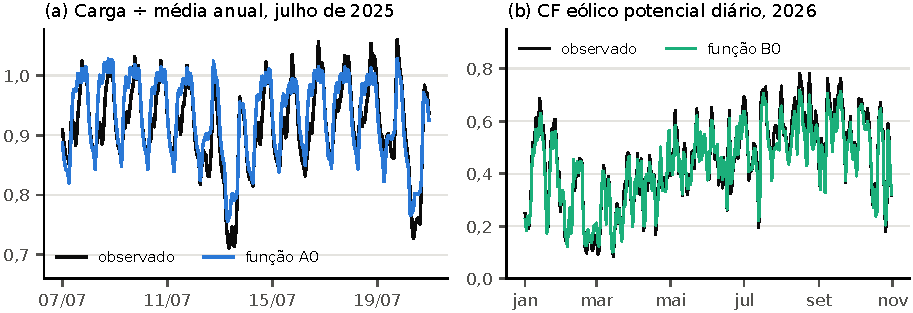
\includegraphics{fig_transferencia}
\caption{Funções de transferência fora do treino: (a) forma da carga em duas semanas de 2025; (b) média diária do CF eólico em 2026.}
\label{fig:transferencia}
\end{figure}

A Figura~\ref{fig:transferencia} compara previsões e observações fora do treino. No CF eólico de 2025, também fora do treino, a correlação horária com o observado é \CorrEol. Nenhuma variável de clima de 1995 a 2021 fica fora da faixa de treino em mais de \Extrap\% das horas, de modo que quase não há extrapolação.

\subsection{Geração hidráulica e térmica}
\label{sec:hidraulica}

A térmica repete a série horária de um dos anos de 2022 a 2025. A hidráulica preserva a energia diária desse mesmo ano, mas a sua distribuição dentro do dia responde à carga líquida, como ocorre no despacho observado (a correlação entre os desvios intradiários das duas é de \CorrHidMin{} a \CorrHidMax{} em 2022--2025):
\begin{equation}
  H(t) = \bar{H}_d + \beta \left[ \ell(t) - \bar{\ell}_d \right],
  \label{eq:hidraulica}
\end{equation}
em que $\bar{H}_d$ é a média do dia, $\ell$ é a carga menos a MMGD e as gerações eólica, solar e térmica, sem cortes, e $\bar{\ell}_d$ é a sua média no dia. O resultado é limitado ao mínimo e ao máximo mensais do ano hidrológico e reajustado para conservar a energia do dia. O coeficiente $\beta$ diminui quando a carga líquida oscila mais: foi de \BetaIni{} em 2022, \BetaVinteCinco{} em 2025 e \BetaCentral{} em 2026. O caso central usa o de 2026, ano observado com a oscilação mais próxima da simulada para 2030.

\subsection{Cenários}
\label{sec:cenarios}

Os cenários combinam quatro níveis de data centers e três de capacidade eólica (Tabela~\ref{tab:cenarios}). A carga sem data centers é a da segunda revisão do PLAN \parencite{plan_2rq} menos a parcela de data centers nela incluída, para que esta não seja contada duas vezes. O cenário alto usa também um inventário de \NProjetosDC{} projetos, levantado em portarias, processos da ANEEL e imprensa setorial. Como a projeção oficial já é expressa em carga na rede, não se aplica o índice de eficiência energética do data center (PUE). O cadastro da ANEEL não informa datas para os projetos fora de operação, e por isso a expansão eólica é definida pela fase dos empreendimentos.

\begin{table}[htb]
\centering
\caption{Níveis adotados para 2030.}
\label{tab:cenarios}
\footnotesize
\renewcommand{\arraystretch}{1.15}
\setlength{\tabcolsep}{4pt}
\begin{tabularx}{\textwidth}{@{}llr>{\raggedright\arraybackslash}X@{}}
\toprule
Dimensão & Cenário & Valor & Definição \\
\midrule
\LinhasCenarios
\bottomrule
\end{tabularx}
\end{table}

\subsection{Simulação de Monte Carlo}
\label{sec:montecarlo}

Cada um dos \NSorteios{} sorteios combina três elementos:
\begin{itemize}
  \item um ano meteorológico entre 1995 e 2025, que define as formas de carga e MMGD e os CFs eólico e solar, dispostos no calendário de 2030;
  \item um ano hidrológico entre 2022 e 2025, que define a energia hidráulica diária e a térmica;
  \item blocos de sete dias de resíduos fora da amostra, das quatro séries em conjunto, tirados de uma janela de 14~dias em torno da mesma época do ano.
\end{itemize}

Os resíduos são necessários porque as funções de transferência estimam médias, com menos variação do que as séries observadas. Eles vêm do período de julho de 2024 a outubro de 2026 e são centrados por mês, para não alterar o nível médio. Com eles, o desvio-padrão horário do CF eólico de 2025, fora da amostra, é \DpSim, contra \DpObs{} observado.

O mesmo sorteio é usado em todos os cenários, o que permite calcular diferenças pareadas. São reportados a média e os percentis 5 e 95 (P5 e P95) dos sorteios. Como estes repetem 31 anos meteorológicos e quatro hidrológicos, aumentar o seu número não reduz a incerteza devida à amostra de anos. Essa incerteza é estimada à parte, por reamostragem dos anos com reposição (4.000 reamostras), e informada como IC95 da média.

A compensação eólica é calculada por dois critérios principais. O primeiro iguala a energia anual dos data centers. O segundo iguala a importação anual à do caso sem data centers, e a capacidade necessária é obtida por bisseção.

\subsection{Classificação dos cortes}
\label{sec:classificador}

Também foi testado um classificador das horas com corte eólico, com variáveis conhecidas antes do evento. Para o corte por razão energética, a área sob a curva precisão-revocação ficou entre \PrMin{} e \PrMax, contra \AcasoMin{} a \AcasoMax{} ao acaso. As probabilidades, porém, não são estáveis: a fração de horas com corte, por qualquer motivo, passou de \HorasCorteIni\% em 2022 para \HorasCorteFim\% em 2025, e o modelo treinado até um ano erra o nível do seguinte. Por isso o classificador não foi aplicado a 2030, e o simulador calcula apenas o excedente.
